\paragraph[QuizziPedia::Front-End::ModelViews\\::MultipleQuestionsModelView]{QuizziPedia::Front-End::ModelViews::MultipleQuestionsModelView}
\begin{figure} [ht]
	\centering
	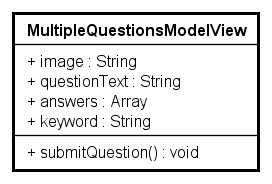
\includegraphics[scale=0.80]{UML/Classi/Front-End/QuizziPedia_Front-end_ModelView_MultipleQuestionsModelView.png}
	\caption{QuizziPedia::Front-End::ModelViews::MultipleQuestionsModelView}
\end{figure} \FloatBarrier
\begin{itemize}
	\item \textbf{Descrizione}: classe di tipo modelview la cui istanziazione è contenuta all'interno della variabile di ambiente \texttt{\$scope} di \textit{Angular\ped{G}}. All'interno di essa sono presenti le variabili e i metodi necessari per il \textit{Two-Way Data-Binding\ped{G}} tra la \textit{view\ped{G}} \texttt{MultipleQuestionsView} e il \textit{controller\ped{G}} \texttt{MultipleQuestionsController}; 
	\item \textbf{Utilizzo}: viene utilizzata per effettuare il \textit{Two-Way Data-Binding\ped{G}} tra la \textit{view\ped{G}} \\\texttt{MultipleQuestionsView} e il \textit{controller\ped{G}} \texttt{MultipleQuestionsController} rendendo disponibili variabili e metodi;
	\item \textbf{Relazioni con altre classi}:
	\begin{itemize}
		\item \textbf{IN \texttt{MultipleQuestionsView}}: \textit{view\ped{G}} contenente le direttive per creare una domanda a risposta multipla; 
		\item \textbf{IN \texttt{MultipleQuestionsController}}: questa classe permette di gestire la creazione e la modifica di una domanda a risposta multipla.
	\end{itemize}
	\item \textbf{Attributi}:
	\begin{itemize}
		\item \texttt{+ image: String} \\ Attributo contenete l'URL dell'immagine caricata dall'utente;
		\item \texttt{+ questionText: String} \\ Attributo contenente il testo della domanda;
		\item \texttt{+ answers: Array}\\ \textit{array} che contiene coppie di valori. Queste coppie sono formate da:
		\begin{itemize}
			\item \texttt{type: String} \\ Indica la tipologia della risposta;
			\item \texttt{text: String} \\ Contiene il testo dell'affermazione;
			\item \texttt{url: String} \\ Rappresenta l'immagine della risposta;
			\item \texttt{attributesForTForMultiple: Mixed} \\ Contiene i seguenti attributi:
			\begin{enumerate}
				\item \texttt{isItRight: Boolean} \\ Contiene se la risposta è vera o falsa.
			\end{enumerate}
		\end{itemize}
		\item \texttt{+ keyword: String} \\ Attributo contenente la keyword associata alla domanda/questionario.
	\end{itemize}
	\item \textbf{Metodi}:
	\begin{itemize}
		\item \texttt{+ submitQuestion(): void}\\ 
		Metodo che gestisce l’evento click sul pulsante di conferma sulla domanda. Raccoglie i dati dal modelview e li manda al server attraverso \texttt{QuestionService}. Poi verrà effettuato il redirect alla pagina di gestione delle domande oppure al questionario che si stava creando.
	\end{itemize}
\end{itemize}

